\documentclass[preprint,12pt,aps,pra,showkeys,amsmath,amssymb,superscriptaddress,floatfix]{revtex4-2}
\usepackage[T1]{fontenc}
\usepackage[utf8]{inputenc}
\usepackage{amsmath,amssymb,amsthm,mathtools,mathrsfs}
\usepackage{microtype,booktabs,enumitem}
\usepackage{xcolor,tikz,etoolbox}
\usepackage[skins,breakable]{tcolorbox}
\usepackage{needspace}
% Keep diagram geometry independent of REVTeX preprint body spacing.
\AtBeginEnvironment{tikzpicture}{\linespread{1}\selectfont}
\usetikzlibrary{arrows.meta,positioning,calc,fit,decorations.pathreplacing}
\usepackage{graphicx}
\usepackage{hyperref}

\definecolor{MMBlue}{RGB}{0,82,155}
\definecolor{MMOrange}{RGB}{200,80,0}
\tikzset{
 mmnode/.style={draw=MMBlue,rounded corners=2pt,fill=MMBlue!4,align=left,execute at begin node={\raggedright},text width=5cm,font=\fontsize{10}{12}\selectfont,inner sep=6pt},
 mmimport/.style={mmnode,draw=black!65,fill=black!4},
 mmcandidate/.style={mmnode,draw=MMOrange,dashed,fill=MMOrange!5},
 mmrejected/.style={mmnode,draw=black,densely dotted,fill=black!8},
 mmproof/.style={->,thick,MMBlue},
 mmflow/.style={->,semithick,black!70},
 mmrepair/.style={->,dashed,thick,MMOrange},
 mmcandidatearrow/.style={->,dashed,semithick,MMOrange},
 mmnote/.style={font=\scriptsize,fill=white,inner sep=2pt,align=center}}

\usepackage[section]{placeins}
\setlength{\emergencystretch}{3em}
\setlist{itemsep=3pt,topsep=4pt}
\newtheorem{theorem}{Theorem}[section]
\newtheorem{proposition}[theorem]{Proposition}
\newtheorem{lemma}[theorem]{Lemma}
\newtheorem{corollary}[theorem]{Corollary}
\theoremstyle{definition}
\newtheorem{definition}[theorem]{Definition}
\newtheorem{example}[theorem]{Example}
\theoremstyle{remark}
\newtheorem{remark}[theorem]{Remark}
% Avoid isolated statement headings and single-line paragraph fragments.
\BeforeBeginEnvironment{theorem}{\Needspace{6\baselineskip}}
\BeforeBeginEnvironment{definition}{\Needspace{5\baselineskip}}
\BeforeBeginEnvironment{proposition}{\Needspace{5\baselineskip}}
\BeforeBeginEnvironment{lemma}{\Needspace{5\baselineskip}}
\BeforeBeginEnvironment{corollary}{\Needspace{5\baselineskip}}
\clubpenalty=5000
\widowpenalty=5000
\newcommand{\R}{\mathbb R}\newcommand{\Z}{\mathbb Z}\newcommand{\N}{\mathbb N}
\newcommand{\Pa}{\operatorname{Pa}}\newcommand{\Desc}{\operatorname{Desc}}
\newcommand{\cl}{\operatorname{cl}}\newcommand{\cost}{\operatorname{cost}}
\newcommand{\status}{\operatorname{status}}
% Faculty cards: a visual rail groups the five faculties within one agent.
% The rail has no arrowhead and does not represent a proof dependency.
\newcommand{\mmfacultybadge}[1]{%
 \node[circle,draw=MMBlue,line width=1pt,fill=white,
 minimum size=7mm,inner sep=0pt,font=\sffamily\small\bfseries,text=MMBlue]
 at ([xshift=15pt,yshift=-15pt]frame.north west) {#1};}
\newcommand{\mmfacultyrail}{%
 \draw[MMBlue!80,line width=1pt]
 ([xshift=15pt,yshift=2pt]frame.north west)--
 ([xshift=15pt,yshift=-2pt]frame.south west);}
\newtcolorbox{mmfacultybox}[2]{enhanced,breakable,
 colback=MMBlue!4,colframe=MMBlue!4,boxrule=0pt,arc=3pt,
 left=39pt,right=9pt,top=4pt,bottom=4pt,
 before skip=2pt,after skip=2pt,
 fontupper=\small\linespread{1.1}\selectfont,
 overlay unbroken={\mmfacultyrail\mmfacultybadge{#1}},
 overlay first={\mmfacultyrail\mmfacultybadge{#1}},
 overlay middle={\mmfacultyrail},overlay last={\mmfacultyrail}}
\newcommand{\mmfaculty}[3]{%
 \begin{mmfacultybox}{#1}{#2}
 {\sffamily\bfseries\color{MMBlue}#2}\par\smallskip #3
 \end{mmfacultybox}}
\newcommand{\agent}[9]{%
 \Needspace{8\baselineskip}
 \subsubsection{#1}
 \noindent\textbf{Object.} #2\par
 \noindent\textbf{Role.} #3\par\smallskip
 \mmfaculty{E}{Ego}{#4}
 \mmfaculty{M}{Memory}{#5}
 \mmfaculty{I}{Intellect}{#6}
 \mmfaculty{S}{Sense}{#7}
 \mmfaculty{A}{Action}{#8}
 \smallskip\noindent #9\par}

\usepackage{longtable,array,calc}
\providecommand{\tightlist}{\setlength{\itemsep}{2pt}\setlength{\parskip}{0pt}}
\makeatletter
\def\frontmatter@abstract@produce{\par\addvspace{\frontmatter@preabstractspace}%
\begingroup\prep@absbox\unvbox\absbox\post@absbox\endgroup
\addvspace{\frontmatter@postabstractspace}}
\makeatother
\newcommand{\field}[2]{\par\smallskip\noindent\textbf{#1.} #2\par}
\setlength{\emergencystretch}{5em}
\AtBeginEnvironment{verbatim}{\small\linespread{1.0}\selectfont}


\hypersetup{colorlinks=true,linkcolor=MMBlue,urlcolor=MMBlue,pdfauthor={Dibakar Sigdel}}

\begin{document}

\title{First-Order Characterization of Convex Minimizers\\[4pt]\large An End-to-End Meta-Math Walkthrough}

\author{Dibakar Sigdel}

\affiliation{Mindverse Computing LLC, Lynnwood, WA 98087, USA}

\date{October 2026}

\begin{abstract}

A supporting affine function supplies global sufficiency. Feasible line
segments supply the converse even when the minimizer is on the boundary.
The report presents the target theorem, declared imports, a dependency
graph, five-faculty node contracts, a continuous proof, a worked
example, and a hypothesis-repair audit. It is an authored mathematical
exposition, not a deployed-agent transcript or a formal proof-assistant
certificate.

\end{abstract}\maketitle\linespread{1.12}\selectfont

\noindent\textbf{ON-01 / Optimization and Numerical Analysis / Report v1}

\section{Target and import contract}

\begin{theorem}

Let \(f:\mathbb R^d\to\mathbb R\) be differentiable and convex, and let
\(C\subset\mathbb R^d\) be nonempty and convex. For \(x_*\in C\), prove
that \(x_*\) minimizes \(f\) over \(C\) if and only if
\(\langle\nabla f(x_*),y-x_*\rangle\ge0\) for every \(y\in C\). In
particular, on \(C=\mathbb R^d\) this is equivalent to
\(\nabla f(x_*)=0\). If \(f\) is strictly convex on \(C\), there is at
most one minimizer.

\end{theorem}

\subsection{Foundations and permitted imports}

Convexity means \(f((1-t)x+ty)\le(1-t)f(x)+tf(y)\) for \(0\le t\le1\);
strict convexity makes it strict for distinct points and \(0<t<1\). Use
differentiation along line segments and the elementary Euclidean inner
product. This is a characterization at a proposed point, not an
existence theorem for arbitrary \(C\).

\clearpage\section{Node interaction workflow}

\begin{center}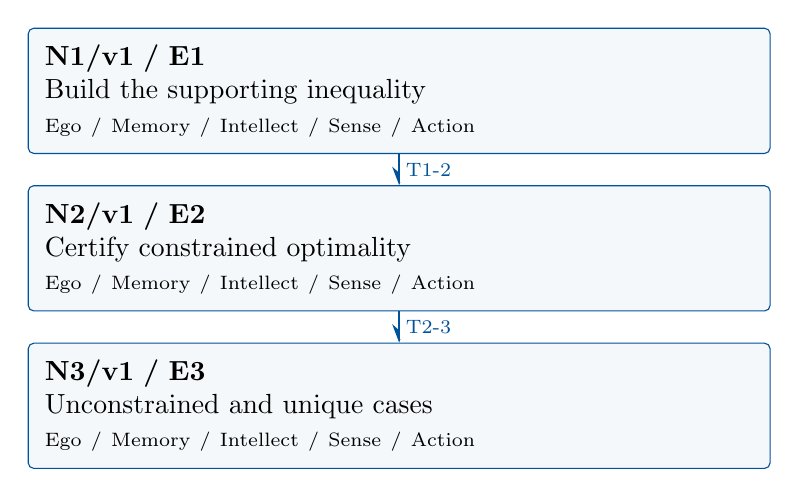
\begin{tikzpicture}[>=Stealth,x=1cm,y=1cm]

\node[mmnode,text width=9cm,minimum height=1.25cm] (N1) at (0,0.0) {\textbf{N1/v1 / E1}\\Build the supporting inequality\\{\scriptsize Ego / Memory / Intellect / Sense / Action}};

\node[mmnode,text width=9cm,minimum height=1.25cm] (N2) at (0,-2.0) {\textbf{N2/v1 / E2}\\Certify constrained optimality\\{\scriptsize Ego / Memory / Intellect / Sense / Action}};

\node[mmnode,text width=9cm,minimum height=1.25cm] (N3) at (0,-4.0) {\textbf{N3/v1 / E3}\\Unconstrained and unique cases\\{\scriptsize Ego / Memory / Intellect / Sense / Action}};

\draw[mmproof] (N1.south) -- node[mmnote,right] {T1-2} (N2.north);

\draw[mmproof] (N2.south) -- node[mmnote,right] {T2-3} (N3.north);

\end{tikzpicture}\end{center}

Each box is one mathematical agent containing all five faculties. Blue
arrows carry the versioned exports listed below. The layout gives a
reading order; only drawn arrows assert dependencies. Diagnostic repair
is separate from the proof DAG.

\subsection{Versioned evidence-transfer ledger}

\begingroup\small\linespread{1.05}\selectfont

\Needspace{5\baselineskip}\field{T1-2: N1/E1/v1 to N2}{\(f(y)\ge f(x)+\langle\nabla f(x),y-x\rangle\).}

\field{Receiving activity}{N2.2}

\field{Compatibility}{E1/v1, convex \(C\), and a proposed \(x_*\in C\). Check: A boundary
minimizer need not have zero gradient; only feasible directions are
tested.}

\Needspace{5\baselineskip}\field{T2-3: N2/E2/v1 to N3}{\(x_*\) is a global minimizer over \(C\) exactly when all feasible
directional inner products are nonnegative.}

\field{Receiving activity}{N3.1}

\field{Compatibility}{E2/v1, and strict convexity when asserting uniqueness. Check: Uniqueness
does not imply existence; for example a function on an open feasible set
can have an unattained infimum.}

\endgroup

\clearpage\section{Agent roles and five-faculty activities}\begingroup\small\linespread{1.05}\selectfont\setlist{itemsep=1pt,topsep=2pt}

\subsection{N1/v1: Build the supporting inequality}

\field{Object and role}{Divide the convex secant inequality by its positive parameter and let it
tend to zero. \textbf{Local obligation:}
\(f(y)\ge f(x)+\langle\nabla f(x),y-x\rangle\).}

\field{Inputs}{Differentiable convex \(f\) and any \(x,y\in\mathbb R^d\).}

\mmfaculty{E}{Ego}{Publish E1/v1 only after establishing this obligation:
\(f(y)\ge f(x)+\langle\nabla f(x),y-x\rangle\).}

\mmfaculty{M}{Memory}{Differentiable convex \(f\) and any \(x,y\in\mathbb R^d\). Retain the
stated assumptions and import versions.}

\mmfaculty{I}{Intellect}{Divide the convex secant inequality by its positive parameter and let it
tend to zero.}

\mmfaculty{S}{Sense}{The parameter approaches zero through positive values; a one-sided
segment is sufficient.}

\mmfaculty{A}{Action}{Carry out activities N1.1--N1.2 below, retaining each calculation and
construction as evidence.}

\smallskip\noindent\textbf{Numbered mathematical activities}

\begin{enumerate}[label=N1.\arabic*,leftmargin=3.4em]

\item For \(0<t\le1\), convexity gives \(f(x+t(y-x))-f(x)\le t(f(y)-f(x))\).
Divide by \(t>0\).

\item Differentiability at \(x\) makes the left quotient tend to
\(\langle\nabla f(x),y-x\rangle\) as \(t\downarrow0\). Rearrangement
yields the supporting inequality for every \(x,y\).

\end{enumerate}

\field{Export E1/v1}{\(f(y)\ge f(x)+\langle\nabla f(x),y-x\rangle\).}

\field{Acceptance gate}{The parameter approaches zero through positive values; a one-sided
segment is sufficient.}

\field{Targeted repair}{If a local Taylor approximation is used as a global lower bound, replace
it by this convexity argument; Taylor's remainder has no automatic sign.
Withhold this export and recheck its descendants after a versioned
correction.}

\clearpage

\subsection{N2/v1: Certify constrained optimality}

\field{Object and role}{Use feasible directional derivatives for necessity and the global
support for sufficiency. \textbf{Local obligation:} \(x_*\) is a global
minimizer over \(C\) exactly when all feasible directional inner
products are nonnegative.}

\field{Inputs}{E1/v1, convex \(C\), and a proposed \(x_*\in C\). Incoming proof
exports: E1/v1 at N2.2.}

\mmfaculty{E}{Ego}{Publish E2/v1 only after establishing this obligation: \(x_*\) is a
global minimizer over \(C\) exactly when all feasible directional inner
products are nonnegative.}

\mmfaculty{M}{Memory}{E1/v1, convex \(C\), and a proposed \(x_*\in C\). Incoming proof
exports: E1/v1 at N2.2. Retain the stated assumptions and import
versions.}

\mmfaculty{I}{Intellect}{Use feasible directional derivatives for necessity and the global
support for sufficiency.}

\mmfaculty{S}{Sense}{A boundary minimizer need not have zero gradient; only feasible
directions are tested.}

\mmfaculty{A}{Action}{Carry out activities N2.1--N2.2 below, retaining each calculation and
construction as evidence.}

\smallskip\noindent\textbf{Numbered mathematical activities}

\begin{enumerate}[label=N2.\arabic*,leftmargin=3.4em]

\item If \(x_*\) minimizes \(f\), then for \(y\in C\) the segment
\(x_*+t(y-x_*)\) remains feasible. Its difference quotient from \(x_*\)
is nonnegative for \(t>0\). Taking the limit gives
\(\langle\nabla f(x_*),y-x_*\rangle\ge0\).

\item Conversely, if those inequalities hold, E1 gives
\(f(y)\ge f(x_*)+\langle\nabla f(x_*),y-x_*\rangle\ge f(x_*)\) for every
\(y\in C\). This is the required global conclusion.

\end{enumerate}

\field{Export E2/v1}{\(x_*\) is a global minimizer over \(C\) exactly when all feasible
directional inner products are nonnegative.}

\field{Acceptance gate}{A boundary minimizer need not have zero gradient; only feasible
directions are tested.}

\field{Targeted repair}{If stationarity is imposed at the boundary, restore the
feasible-direction inequality instead of demanding all directions have
zero derivative. Withhold this export and recheck its descendants after
a versioned correction.}

\clearpage

\subsection{N3/v1: Unconstrained and unique cases}

\field{Object and role}{Test the negative gradient as a direction, and use a midpoint to rule
out two distinct minimizers. \textbf{Local obligation:} For
\(C=\mathbb R^d\), zero gradient is equivalent to optimality; strict
convexity gives at most one minimizer.}

\field{Inputs}{E2/v1, and strict convexity when asserting uniqueness. Incoming proof
exports: E2/v1 at N3.1.}

\mmfaculty{E}{Ego}{Publish E3/v1 only after establishing this obligation: For
\(C=\mathbb R^d\), zero gradient is equivalent to optimality; strict
convexity gives at most one minimizer.}

\mmfaculty{M}{Memory}{E2/v1, and strict convexity when asserting uniqueness. Incoming proof
exports: E2/v1 at N3.1. Retain the stated assumptions and import
versions.}

\mmfaculty{I}{Intellect}{Test the negative gradient as a direction, and use a midpoint to rule
out two distinct minimizers.}

\mmfaculty{S}{Sense}{Uniqueness does not imply existence; for example a function on an open
feasible set can have an unattained infimum.}

\mmfaculty{A}{Action}{Carry out activities N3.1--N3.2 below, retaining each calculation and
construction as evidence.}

\smallskip\noindent\textbf{Numbered mathematical activities}

\begin{enumerate}[label=N3.\arabic*,leftmargin=3.4em]

\item In the unconstrained case substitute \(y=x_*-\nabla f(x_*)\) in E2 to
get \(-\|\nabla f(x_*)\|^2\ge0\), hence the gradient is zero. The
converse follows immediately from E2.

\item If distinct \(x_*,z_*\) both minimize and \(f\) is strictly convex on
\(C\), their midpoint lies in \(C\) and has strictly smaller value than
the average of their equal minimum values, a contradiction. This proves
at-most-one, completing the theorem.

\end{enumerate}

\field{Export E3/v1}{For \(C=\mathbb R^d\), zero gradient is equivalent to optimality; strict
convexity gives at most one minimizer.}

\field{Acceptance gate}{Uniqueness does not imply existence; for example a function on an open
feasible set can have an unattained infimum.}

\field{Targeted repair}{If a unique minimizer is declared without an existence argument, retain
the precise at-most-one conclusion. Withhold this export and recheck its
descendants after a versioned correction.}

\endgroup\clearpage\section{Continuous mathematical proof}\label{sec:proof}

\subsection{N1 --- Build the supporting
inequality}\label{n1-build-the-supporting-inequality}

\begin{enumerate}
\def\labelenumi{\arabic{enumi}.}
\item
  \textbf{N1.1.} For \(0<t\le1\), convexity gives
  \(f(x+t(y-x))-f(x)\le t(f(y)-f(x))\). Divide by \(t>0\).
\item
  \textbf{N1.2.} Differentiability at \(x\) makes the left quotient tend
  to \(\langle\nabla f(x),y-x\rangle\) as \(t\downarrow0\).
  Rearrangement yields the supporting inequality for every \(x,y\).
\end{enumerate}

\subsection{N2 --- Certify constrained
optimality}\label{n2-certify-constrained-optimality}

\begin{enumerate}
\def\labelenumi{\arabic{enumi}.}
\item
  \textbf{N2.1.} If \(x_*\) minimizes \(f\), then for \(y\in C\) the
  segment \(x_*+t(y-x_*)\) remains feasible. Its difference quotient
  from \(x_*\) is nonnegative for \(t>0\). Taking the limit gives
  \(\langle\nabla f(x_*),y-x_*\rangle\ge0\).
\item
  \textbf{N2.2.} Conversely, if those inequalities hold, E1 gives
  \(f(y)\ge f(x_*)+\langle\nabla f(x_*),y-x_*\rangle\ge f(x_*)\) for
  every \(y\in C\). This is the required global conclusion.
\end{enumerate}

\subsection{N3 --- Unconstrained and unique
cases}\label{n3-unconstrained-and-unique-cases}

\begin{enumerate}
\def\labelenumi{\arabic{enumi}.}
\item
  \textbf{N3.1.} In the unconstrained case substitute
  \(y=x_*-\nabla f(x_*)\) in E2 to get \(-\|\nabla f(x_*)\|^2\ge0\),
  hence the gradient is zero. The converse follows immediately from E2.
\item
  \textbf{N3.2.} If distinct \(x_*,z_*\) both minimize and \(f\) is
  strictly convex on \(C\), their midpoint lies in \(C\) and has
  strictly smaller value than the average of their equal minimum values,
  a contradiction. This proves at-most-one, completing the theorem.
\end{enumerate}

\hfill$\square$

\section{Worked orchestration}

For \(f(x)=(x+1)^2\) and \(C=[0,\infty)\), choose \(x_*=0\). The
derivative is \(2\), not zero, but \(f'(0)(y-0)=2y\ge0\) for all
feasible \(y\). The theorem certifies the boundary minimizer; strict
convexity makes it unique.

\subsection{Boundary and hypothesis audit}

Without convexity of \(f\), zero gradient need not indicate a minimum:
\(f(x)=-x^2\) has \(f'(0)=0\) and a strict maximum at zero. Existence
also fails for the strictly convex \(f(x)=x^2\) on \(C=(0,1)\), whose
infimum is not attained.

\section{Illustrative failure and repair}

The following is an authored diagnostic scenario. Changed assumptions
define a new contract; they do not retroactively prove the original
statement.

\subsection{Rejected argument, diagnosis, and correction}
\textbf{Rejected N2 claim:} a constrained optimum must satisfy
\(\nabla f=0\). The worked boundary example refutes it.
\textbf{Diagnosis:} Intellect tested infeasible negative directions.
\textbf{Repair:} test only \(y-x_*\) with \(y\in C\) and prove the
variational inequality. This replaces the invalid candidate with the
exact §1 statement; the unconstrained zero-gradient corollary still
holds separately.

\subsection{Publication and reuse}
The corrected export retains its explicit assumptions. A hypothetical
revision receives a new version, and each consuming activity is
rechecked; this scenario is not a recorded runtime event. \textbf{Next
direction:} Add normal cones or convex inequality constraints to develop
constrained optimality without confusing boundary points with
unconstrained stationary points.

\par\medskip\begingroup\small\linespread{1.0}\selectfont\noindent\textbf{Provenance.} This authored proof is complete relative to its declared imports. Reuse
each export with its assumptions, proof, and version. The original
Markdown remains available for comparison.
\par\endgroup

\par\smallskip\begingroup\small\linespread{1.0}\selectfont\noindent\textbf{Further reading.} \href{https://web.stanford.edu/~boyd/cvxbook/}{Boyd and Vandenberghe,
Convex Optimization} for convexity, optimality, and descent;
\href{https://www.math.umd.edu/~mariakc/Spring2020Class.html}{University
of Maryland, Scientific Computing I} for the numerical-analysis setting.
The estimates used here are derived explicitly in §4.\par\endgroup

\end{document}
